\chapter{螺旋线型行波管的改进}
由于螺旋线型行波管具有宽频带,高增益,轻重量、小体积(由于采用了周期永磁聚束,重量和体积比以前减小了许多)低噪声、长寿命等特点,因而在地面接力通信、卫星通信、雷达、电子对抗以及微波测试等设备中获得了广泛的应用。近年来,为了满足上述各方面应用对行波管的要求,人们作了很多改进工作,使行波管的性能有了很大的提高。例如,有的做到了大于倍频程(甚至达到8:1)的频宽;有的做到了60\textasciitilde70分贝的高增益,有的做到了良好的线性度;有的做到了低达1分贝的噪声系数;有的和电源一起做成了小型化的行波管放大器;还有的由于做到了几十万小时的长寿命和40\%以上的高效率而被用到卫星上……等等。目前,从功率来看,螺旋线型行波管已能做到连续波输出1千瓦,而从频率来看则可以覆盖整个厘米波段和毫米波段

对于中小功率螺旋线型行波管来说,这些改进工作概括起来是从下面这几方面着手的。
\subsection{提高可靠性和延长寿命}
从整机角度来看,要求所用的元件和器件具有高的可靠性和长的寿命,这无论对于地面接力通信以及卫星通信用的行波管来说,都具有头等重要的意义。地面接力通信虽然可以更换管子,但是由于一条通信线路往往有几千公里长、几十个接力站、上百个行波管,因此其中只要有一只行波管损坏,就会使整个通信线路中断。在卫星通信中,如果卫星上的行波管损,那么不但会使整个通信中断,而且无法更换或修复。因此年来高可靠性、长寿命的要求已被列为重要的研究课题。目前为保证高可靠性和长寿命所采取的措施有:严格的工艺卫生和工艺操作,例如提高排气时的烘箱烘烤温度,使零件彻底去气:延长排气时间使管内零件充分出气;采用无油真空系统排气,以避免油蒸气污染,提高真空度;管内附加高效率的吸气剂(如锆铝吸气剂、锆石墨吸气剂等)吸走残余气体,提高真空度;研制长寿命阴极;用离子阱结构防止正离子回轰阴极表面等等。此外还应对行波管进行严格的筛选,剔除初期失效的管子,以提高可靠性。采用上述措施后,行波管的寿命可以大大延长。卫星行波管的寿命一般是几万到十几万小时。

为了使大家了解初期失效是怎么回事,我们对行波管的失效规律作一简单介绍。

大量实践证明,行波管的失效情况(用失效率来表示)与时间的关系是一条两头高、中间低的“浴盆曲线”,如图\ref{ch13-1}所示。
\begin{figure}[phtb]
	\centering
	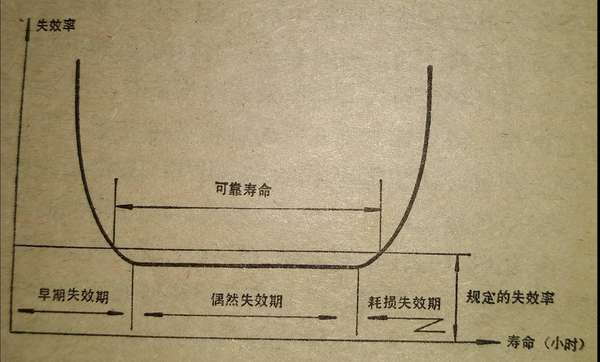
\includegraphics[width=0.52\linewidth]{figure/ch13-1}
	\caption{典型的行波管失效曲线}
	\label{ch13-1}
\end{figure}

由图可见,行波管的失效率随工作时间的变化大致可分为三个阶段。

(1)早期失效期。出现在管子工作的初期,特点是失效率较高,但失效率随着时间的增加将迅速下降。造成早期失效的原因主要是零件、材料有缺陷,制管工艺的漏洞(真空卫生、操作、设备等控制不严等)及在工厂中未被发现的制造上的缺陷等。表现在灯丝断路、电极短路、漏气、阴极受损伤等。期除早期失效的主要方法就是进行筛选,筛选的时间要根据具体的管子、具体的要求经实验决定。如卫星行波管由于要求较高,筛选的时间就较长(达2000小时至4000小时)

(2)偶然失效期。出现在早期失效期之后,特点是失效率低且稳定,近似为一常数,与时间的变化关系不大,是行波管稳定工作的阶段。这个阶段的失效是偶然因素引起的。

偶然失效期的长短决定了行波管的寿命长短,因此,开展行波管的长寿命工作主要是为了延长它的偶然失效期。

(3)耗损失效期(或称老化失效期)。出现在行波管使用的后期。同一批管子在差不多的时间内失效,失效率随时间迅速上升。耗损失效期所发生的故障很少是机械的和人为的故障,大部分是以散焦、阴极发射差、输出功率下降……等特性恶化的形式出现,其形成原因主要是阴极的耗损。

阴极的耗损除了阴极本身的内在质量问题(如基金属、活性物质、激活剂等的质量和工艺处理)以外,外部工作环境也是一个重要原因。阴极损坏的外部原因主要是管内真空度不良。管内真空度不良使得阴极很容易中毒,同时还可能产生很多正离子,正离子轰击阴极就要产生离子斑,使阴极发射不均匀,而发射不均匀将导致局部发射面的负荷过重,发射电流密度急剧增大,最后阴极全部损坏。另一个原因是阴极蒸发大、活性物质消耗严重,这常常是因阴极工作温度过高引起的,因此和灯丝有关。
\subsection{提高效率}
一般行波管的效率在15\textasciitilde20\%以下,为了得到几瓦的输出功率,就需要消耗几十瓦的电源功率,这是很不经济的。为什么行波管的效率比较低呢?我们知道,行波管的放大是依靠电子束和高频场相互作用、交换能量来实现的,电子由于交出了能量,它的速度就要降低,因而就不能和高频场在整个作用距离内始终保持同步。这些电子虽然已经不能有效地把能量继续交出来,然而它们的速度(动能)仍然很高,全变成了收集极处的热能,这就决定了行波管的效率较低。有没有办法使它们在整个作用距离内始终保持同步呢?有的。办法之一是改变螺旋线的螺距,因而改变慢波系统的相速,使螺旋线的螺距逐渐变小,其相速也就随之减小,这样它就能和因给出能量而逐渐减速的电子继续保持同步,在较长的距离内有效地交换能量。这个办法称为速度渐变法。办法之二是维持螺旋线的螺距不变,也就是维持相速不变,而把螺旋线分段,上面加以不同的电压,靠近输出端的那段,其所加的电压要比靠近输入端那段的电压高。因给出能量而减速的电子在输出端段螺旋线电压的加速下,提高了速度,因而能和高频场继续保持同步。这个办行波管的功率耗散主要是消耗在收集极上的功率耗散,因法称为电压跳变法。

此如果降低收集极电压就能提高效率,这是显而易见的。目前已广泛地采用了多级降压收集极的办法来进一步提高效率。此外,还可以采取其他的一些措施来提高效率,如改善旋线的散热、减小螺旋线的损耗,提高灯丝的热效率,改善聚束等等这里就不多讲了。

由于采取了上面的一系列措施,目前行波管的效率已经能做到40\%\textasciitilde70\%了。
\subsection{展宽频带}
螺旋线型行波管的突出特点就是频带很宽,这主要是因为慢波系统螺旋线本身是弱色散的。如果我们再增加一些辅助措施,就会使频带变得更宽。例如,可以在螺旋线外加上一个轴向导电的屏蔽筒,并使它靠近螺旋线,就可以改善螺旋线的色散特性,展宽频带。目前已有做到8:1倍频程(例如2\textasciitilde16千兆赫)的行波管。
\subsection{提高增益}
高增益虽是行波管的一个优点,但在某些领域里又对它提出了更高的要求。例如,在雷达发射机前级固态振荡源输出较小的情况下,为了推动大功率的末级放大管,就需要增益大于50分贝的行波管。

阻碍增益提高的一个主要障碍是自激振荡,因此,为了提高增益,要求很好地改进输能装置和集中衰减器的匹配,以防止自激振荡的产生。此外,还可以采取提高螺旋线的精度、抑止收集极二次电子的返回、进一步提高导流系数等办法来提高行波管的增益。
\subsection{减轻重量、缩小体积}
随着行波管在空间技术和军事等方面的应用,对它提出了轻和小的要求。近年来,由于采用了新材料,新工艺而获得了较大的进展。我们知道,整个行波管中磁系统对其重量和体积起着举足轻重的作用。周期永磁聚束系统的出现,使行波管的重量和体积大为缩小。近年来又进一步出现了高磁能积的磁性材料,如钐钴磁钢,它的磁能积为铝镍钴磁钢的四倍,而重量仅是它的四分之一,因而使得磁系统的重量和体积进一步缩小。例如,$ X $波段20瓦的行波管的饱和增益近40分贝,其体积仅$ 9\times19\times130 $立方毫米,可以放到X波段标准波导中去重量不到200克。另外,还有的把电源集成化,然后与行波管组成一体,它的重量轻,体积也很小。
\subsection{改善非线性特性}
行波管的非线性包括幅度非线性和相位非线性。目前特别是相位非线性问题更为人们所关心。一般的螺旋线型行波管其螺旋线电压变化1\%将引起输出信号相位$ \SI{20}{\degreeCelsius}\textasciitilde\SI{50}{\degreeCelsius} $的变化这在一般情况下还是能够允许的,但是,在一些新型雷达中这样的相位稳定性却会使雷达无法工作。为了提高相位稳定性,我们采取的改进办法是缩短电子在螺旋线中飞行的距离也就是缩短螺旋线的长度,更确切地说应该是减小$ N $(即$ \frac{l}{\lambda_g} $)数。从增益计算公式$ G = A +\mathit{BCN}-6 $(参看第\ref{ch4}章)中我们可以看出,如果减小$ N $,则为了保持同样的$ G $就需要增大导流系数$ P_\theta $以提高增益参量$ C $,有的管子$ P_\theta $,已做到高达10微朴以上,这样,相位稳定性就可以提高几倍,行波管长度也可以缩短很多。当然,在工艺上和设计上都会增加很多困难。
\subsection{多信号放大}
目前,很多雷达往往采用多频率体制,这就要求行波管能够同时放大几个频率的信号(它们之间频率略有差异),每个信号都要有较大的输出功率,而且相互影响(即所谓“交叉调制”)要小。因此,行波管的线性动态范围应该比较宽,这是设计这类管子时需要注意的。
\subsection{改进散热技术}
采用氧化铍、氮化硼等新型陶瓷材料来做螺旋线的夹持杆,并使之与螺旋线及外屏蔽筒(金属管壳)焊接起来,可以大大提高螺旋线的散热能力因而提高螺旋线型行波管的功率。
\subsection{应用电子计算机设计行波管}
目前,电子计算机已被广泛地用来设计行波管的高频系统、电子枪、聚束系统等部件,收到了快速准确的效果。电子计算机还可以对行波管的大信号工作状态、降压收集极以及新型慢波系统的色散特性等进行设计计算。